\documentclass[11pt]{extarticle}	 %This allows us to use smaller font sizes
\usepackage{graphicx}
\usepackage[left=0.2cm, right=0.3cm, top=.4cm, bottom= 1.3cm]{geometry} % always specify in print settings to capture entire image
\usepackage{bm}
\usepackage{marvosym} % Sweet symbols, can use for numbering equations
\usepackage{siunitx}
\usepackage{caption}
\usepackage{wrapfig}
\usepackage{dsfont} % \mathds{1} for characteristic function
\usepackage{bbm} %\mathbbm{1} for characteristic function
\usepackage{amsmath}
\usepackage{mathtools}
\usepackage{commath}
\usepackage{color}
\newcommand*{\mathcolor}{}
\def\mathcolor#1#{\mathcoloraux{#1}}
\newcommand*{\mathcoloraux}[3]{
  \protect\leavevmode
  \begingroup
    \color#1{#2}#3
\endgroup}
\usepackage{hyperref}
\usepackage{amssymb}
\usepackage[utf8]{inputenc}
\usepackage{enumitem}
\usepackage{physics}		%Bra-Kets for QM
\usepackage{xcolor}
\usepackage{nicefrac}
\usepackage{mathrsfs}
\usepackage{tikz}
\usetikzlibrary{3d,calc,patterns,angles,quotes}
\usepackage{tikz-3dplot}
\usepackage{pgfplots}
\usepackage{graphicx}
\usepackage{tensor}			% For Tensor objects
\usepackage{subcaption}
\graphicspath{{Template}}	% Update this to specify problem set folder name for graphics reference
\let\oldL\L
\renewcommand\L{\mathcal{L}}
\newcommand{\Z}{\mathbb{Z}}
\newcommand{\N}{\mathbb{N}}
\newcommand{\R}{\mathbb{R}}
\newcommand{\DS}{\displaystyle}
\newcommand\numberthis{\addtocounter{equation}{1}\tag{\theequation}}
\pgfplotsset{compat=1.8}
\makeatletter
\newcommand*\dotp{\mathpalette\dotp@{.5}}
\newcommand*\dotp@[2]{\mathbin{\vcenter{\hbox{\scalebox{#2}{$\m@th#1\bullet$}}}}}
\makeatother
\allowdisplaybreaks % allows equations to break up between pages.
\begin{document}
\setlength{\belowdisplayskip}{2pt} \setlength{\belowdisplayshortskip}{2pt}
\setlength{\abovedisplayskip}{2pt} \setlength{\abovedisplayshortskip}{2pt}
\begin{flushright}
\textsc{Channel Capacities\newline}				% Sudent ID
\end{flushright}
\vspace{-\baselineskip}\vspace{-\baselineskip}
\begin{flushleft}
\begin{enumerate}		% begins labels of questions, use (\Alph*) for letters and (\Roman*) for roman numerals

\item

\begin{enumerate}[label=(\Alph*)]
\item
For a classical bit channel with bit flip error probability $p$, it is clear that at $p = \frac{1}{2}$. We deomonstrate this by making the abstraction black-white pixel $\sim$ bit and passing each through a channel with the the desired statistical properties with varying levels of redundancy (duplications of each bit).


\item

  The case where we consider a quantum channel with classical information is nontrivial. In our project we attempted to implement the channel description of the paper {\it Quasi-Superactivation of Classical Capacity of Zero-Capacity Quantum Channels- Laszlo Gyongyosi, Sandor Imre} \url{https://arxiv.org/abs/1206.5693}. We seek to verify the claims of this paper by explicitly constructing the described channel:

\begin{figure}[h]
\centering
\caption{Left side depics the quantum channel $\mathcal{M} = \mathcal{N}_1 \circ \mathcal{N}_2$ where $\mathcal{N}$ is any quantum channel that outputs a maximally mixed state and $\mathcal{N}$ is a $1 \to 2 $ cloning channel (further details with simulated emission), also $F = \frac{2}{3} + \frac{1}{3N}$ where $F = \bra{\psi} \rho \ket{\psi}$.}
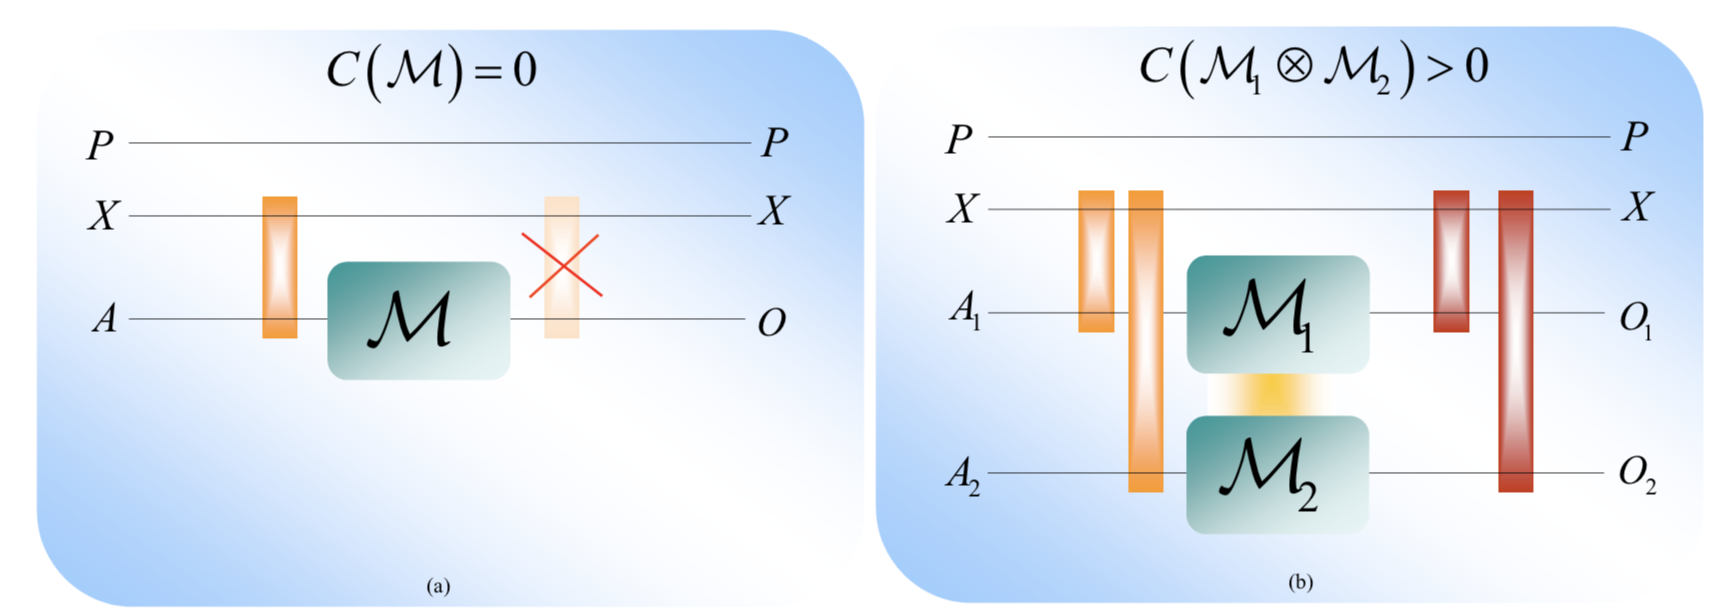
\includegraphics[width=400pt]{first.png}
\caption{As a single channel, this has zero classsical information capacity. Which we test. But, when combining two channels with entangled inputs into the channel $\mathcal{N}_2$, we get non-zero channel capacity.}
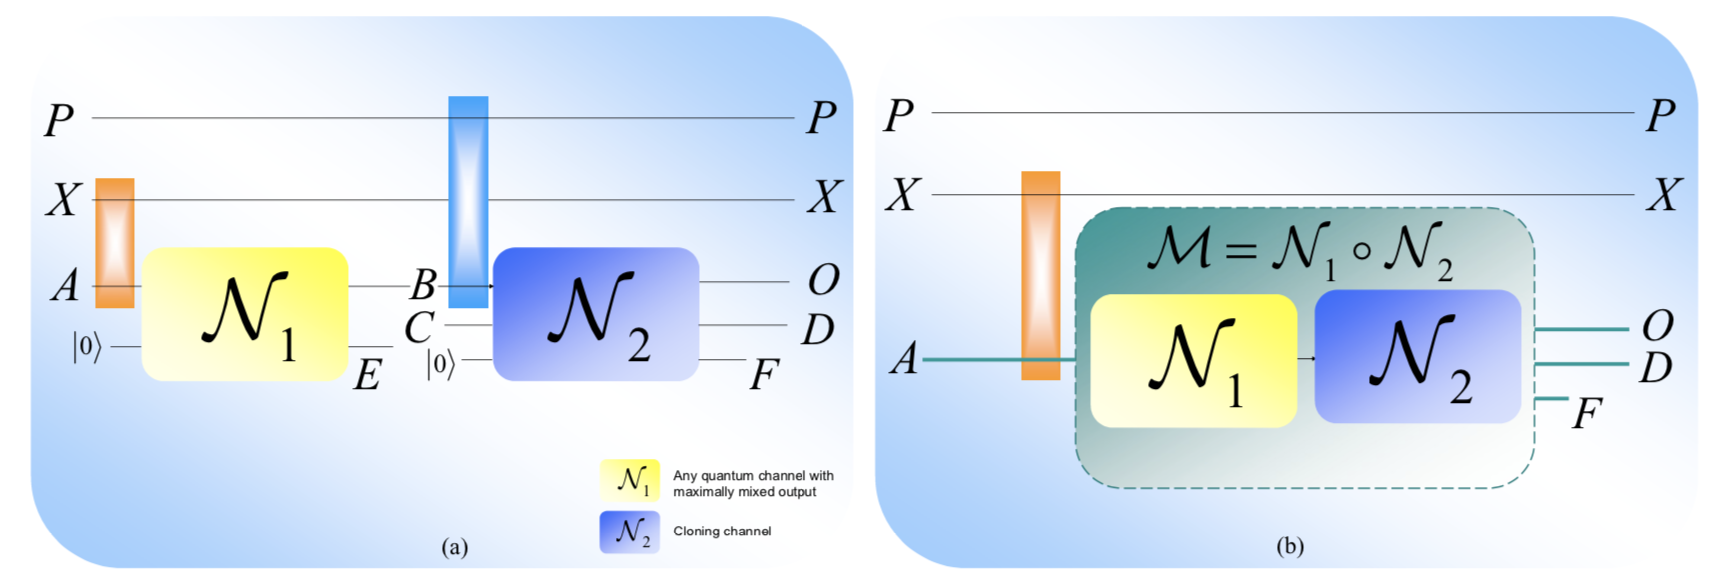
\includegraphics[width=400pt]{second.png}
  \end{figure}
\begin{figure}[h]
  \centering
\caption{Plot of the product channel capacity as a function of the correlation coefficient $\Omega$. When the entaglement coefficient is $\frac{1}{2}$, (so the entangled states input is ) $ \frac{1}{\sqrt{2}} (\ket{0,0} + \ket{11})$. Then there is no quantum correlation that is able to pass through the network and all information is lost. }
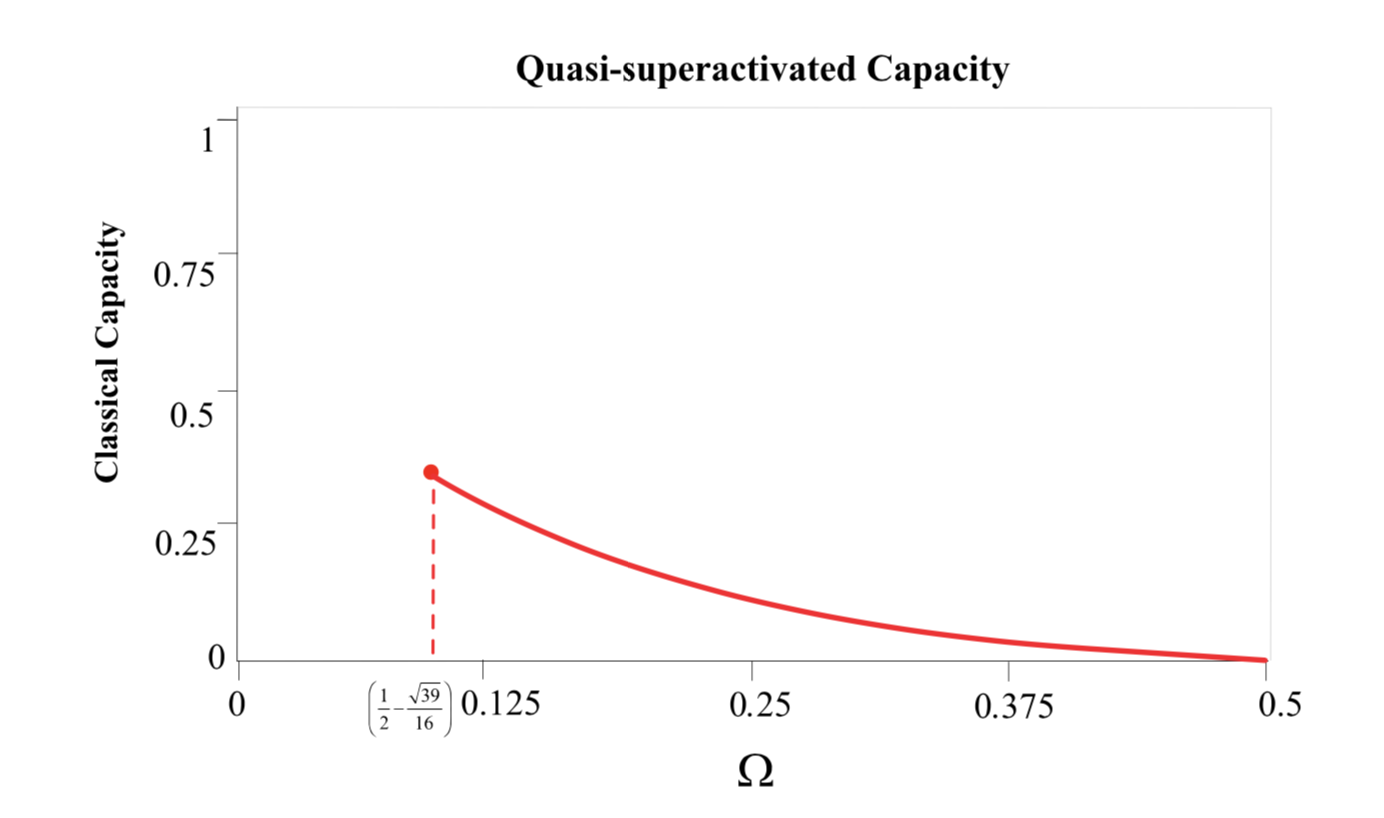
\includegraphics[width=400pt]{correlation.png}
  \end{figure}





\end{enumerate}


\end{enumerate}
\end{flushleft}
\end{document}
